\documentclass[
	12pt, %Schriftgröße
	a4paper,
	liststotoc, %Inhaltsverzeichniseinträge für Listen (z.B. Abbildungen)
	bibtotoc,%Inhaltsverzeichniseinträge f+r Quellen 
	pointlessnumbers, %Entfernt Punkt hinter Gliederungsnummern
	english, %Sprachpaket
	headsepline, %Headertrennlinie
	%footsepline, %Footertrennlinie
	oneside %einseitiges Druckformat %%% Unterdrücken der leeren Seite nach Titelblatt
	]{scrbook} %Dokumentenklasse (Koma-Script)
\usepackage[T1]{fontenc}
\usepackage{float}
\usepackage[utf8]{inputenc}
\usepackage[english]{babel}
\usepackage{lmodern}
\usepackage{markdown}
\usepackage{chronology}
\usepackage{url}
\usepackage{graphicx} %Bilder einfügen
\usepackage{float}
\usepackage{microtype}
\usepackage[a4paper, margin=1in, headsep=2cm]{geometry}
\usepackage[right]{eurosym} %Euro-Zeichen
\usepackage{amssymb}
\usepackage{babel}
\usepackage{fontenc}
\usepackage{graphicx}
\usepackage{cite} %Quellenangaben
\usepackage[numbers]{natbib}
\usepackage{pdflscape}
\usepackage{pdfpages}
\usepackage{scrhack}
\usepackage{breakurl}
\usepackage{bookmark}
\def\UrlBreaks{\do\/\do-}

\usepackage{setspace} % Zeilenabstand
\usepackage[figure]{hypcap}
\usepackage[toc,page]{appendix}
%\usepackage[titletoc]{appendix}
\usepackage[english]{translator}
\usepackage{listings,xcolor} %Codeanzeige
\lstdefinestyle{interfaces}{
  float=tp,
  floatplacement=tbp,
  abovecaptionskip=-5pt
}

%\usepackage[nottoc,numbib]{tocbibind}
\usepackage[normalem]{ulem}
\useunder{\uline}{\ul}{}
\usepackage{pdfpages}
\usepackage{color}
\definecolor{lst-gray}{rgb}{0.98,0.98,0.98}
\definecolor{lst-blue}{RGB}{40,0.0,255}
\definecolor{lst-green}{RGB}{65,128,95}
\definecolor{lst-red}{RGB}{200,0,85}

\onehalfspacing

\lstset{literate=
  {á}{{\'a}}1 {é}{{\'e}}1 {í}{{\'i}}1 {ó}{{\'o}}1 {ú}{{\'u}}1
  {Á}{{\'A}}1 {É}{{\'E}}1 {Í}{{\'I}}1 {Ó}{{\'O}}1 {Ú}{{\'U}}1
  {à}{{\`a}}1 {è}{{\`e}}1 {ì}{{\`i}}1 {ò}{{\`o}}1 {ù}{{\`u}}1
  {À}{{\`A}}1 {È}{{\'E}}1 {Ì}{{\`I}}1 {Ò}{{\`O}}1 {Ù}{{\`U}}1
  {ä}{{\"a}}1 {ë}{{\"e}}1 {ï}{{\"i}}1 {ö}{{\"o}}1 {ü}{{\"u}}1
  {Ä}{{\"A}}1 {Ë}{{\"E}}1 {Ï}{{\"I}}1 {Ö}{{\"O}}1 {Ü}{{\"U}}1
  {â}{{\^a}}1 {ê}{{\^e}}1 {î}{{\^i}}1 {ô}{{\^o}}1 {û}{{\^u}}1
  {Â}{{\^A}}1 {Ê}{{\^E}}1 {Î}{{\^I}}1 {Ô}{{\^O}}1 {Û}{{\^U}}1
  {Ã}{{\~A}}1 {ã}{{\~a}}1 {Õ}{{\~O}}1 {õ}{{\~o}}1
  {œ}{{\oe}}1 {Œ}{{\OE}}1 {æ}{{\ae}}1 {Æ}{{\AE}}1 {ß}{{\ss}}1
  {ű}{{\H{u}}}1 {Ű}{{\H{U}}}1 {ő}{{\H{o}}}1 {Ő}{{\H{O}}}1
  {ç}{{\c c}}1 {Ç}{{\c C}}1 {ø}{{\o}}1 {å}{{\r a}}1 {Å}{{\r A}}1
  {€}{{\euro}}1 {£}{{\pounds}}1 {«}{{\guillemotleft}}1
  {»}{{\guillemotright}}1 {ñ}{{\~n}}1 {Ñ}{{\~N}}1 {¿}{{?`}}1
}

\usepackage{color}

% TC:incbib
% init word counter
\newcommand{\quickwordcount}[1]{%
  \immediate\write18{texcount -1 -sum -merge -q -relaxed #1.tex > #1-words.sum }%
  \input{#1-words.sum}words%
}
\newcommand*{\fullref}[1]{\hyperref[{#1}]{\autoref*{#1} \nameref*{#1}}}

%Hinzufügen von Json 
\colorlet{punct}{red!60!black}
\definecolor{background}{HTML}{EEEEEE}
\definecolor{delim}{RGB}{20,105,176}
\colorlet{numb}{magenta!60!black}

\lstdefinelanguage{json}{
    basicstyle=\normalfont\ttfamily,
    numbers=left,
    numberstyle=\scriptsize,
    stepnumber=1,
    numbersep=8pt,
    showstringspaces=false,
    breaklines=true,
    frame=lines,
    backgroundcolor=\color{background},
    literate=
     *{0}{{{\color{numb}0}}}{1}
      {1}{{{\color{numb}1}}}{1}
      {2}{{{\color{numb}2}}}{1}
      {3}{{{\color{numb}3}}}{1}
      {4}{{{\color{numb}4}}}{1}
      {5}{{{\color{numb}5}}}{1}
      {6}{{{\color{numb}6}}}{1}
      {7}{{{\color{numb}7}}}{1}
      {8}{{{\color{numb}8}}}{1}
      {9}{{{\color{numb}9}}}{1}
      {:}{{{\color{punct}{:}}}}{1}
      {,}{{{\color{punct}{,}}}}{1}
      {\{}{{{\color{delim}{\{}}}}{1}
      {\}}{{{\color{delim}{\}}}}}{1}
      {[}{{{\color{delim}{[}}}}{1}
      {]}{{{\color{delim}{]}}}}{1},
}

\usepackage{chngcntr}
\usepackage{verbatim}
\usepackage{wrapfig}
\counterwithout{figure}{chapter}
\counterwithout{table}{chapter}
\usepackage[toc, acronym, nonumberlist, nogroupskip, shortcuts]{glossaries-extra}
% \usepackage{mathptmx} % times new roman font schriftart
 
\definecolor{mygreen}{rgb}{0,0.6,0}
\definecolor{mygray}{rgb}{0.5,0.5,0.5}
\definecolor{mymauve}{rgb}{0.58,0,0.82}

\lstset{ %
  backgroundcolor=\color{white},   % choose the background color
  basicstyle=\footnotesize,        % size of fonts used for the code
  breaklines=true,                 % automatic line breaking only at whitespace
  captionpos=b,                    % sets the caption-position to bottom
  commentstyle=\color{mygreen},    % comment style
  escapeinside={\%*}{*)},          % if you want to add LaTeX within your code
  keywordstyle=\color{blue},       % keyword style
  stringstyle=\color{mymauve},     % string literal style
}
%%%%%%%%%%%%%%%%%%%%%%%%%%%%%%%%%%%%%%%%%%%%%%%%%%%%%
%%%%%%%%%%% Sonderformatierung
%%%%%%%%%%%%%%%%%%%%%%%%%%%%%%%%%%%%%%%%%%%%%%%%%%%%%

% Seitenabstände für Titelblatt definieren
\geometry{verbose,tmargin=1cm,bmargin=2cm,lmargin=3cm,rmargin=3cm} 

% Hurenkinder und Schusterjungen verhindern (Ja, das heißt wirklich so!!)
\clubpenalty = 10000 \widowpenalty = 10000 \displaywidowpenalty = 10000 

\newcommand{\footfigref}[1]{\footnote{Fig. \ref{#1} on page \pageref{#1}}}

%% Bei Referenzen im Text wird jetzt bei allen Ebenen "Kapitel" vorgestellt, z.b. Kapitel 2, Kapitel 2.2, Kapitel 6.3.2
% \addto\extrasngerman{%
%     \def\sectionautorefname{Kapitel}%
%     \def\subsectionautorefname{Kapitel}%
%     \def\subsubsectionautorefname{Kapitel}%
%     }

% Vertikaler Abstand zwischen Ende Textblock - Ende Fußzeile --> Abstand der Seitenzahl von Rand erhöhen 
\setlength{\footskip}{10mm}

% Abstand vor/nach Überschriften verändern

\RedeclareSectionCommand[%
    beforeskip=0\baselineskip,
    afterskip=0.5\baselineskip
]{chapter}

\RedeclareSectionCommand[%
    beforeskip=0.5\baselineskip,
    afterskip=0.5\baselineskip
]{section}

\RedeclareSectionCommand[%
    beforeskip=0.1\baselineskip,
    afterskip=0.1\baselineskip
]{subsection}

\RedeclareSectionCommand[%
    beforeskip=0.01\baselineskip,
    %%afterskip=0.2\baselineskip
]{paragraph}

\setlength{\abovecaptionskip}{4pt}  % 1pc=12pt 
\setlength{\belowcaptionskip}{0pt}
%\setlength{\textfloatsep}{4pt}
\setlength{\intextsep}{1pc}
\setlength{\headheight}{28.72635pt}

%% Verkleinerung der Textgröße unter Abbildungen
\addtokomafont{caption}{\small}

% Den Punkt am Ende der Glossareinträge deaktivieren
\renewcommand*{\glspostdescription}{}

%Glossar-Befehle anschalten

% sorgt dafür, dass bei Leerzeile die Einrückung verhindert und stattdessen eine Leerzeile eingefügt wird % erspart bigskips und erhöht die Lesbarkeit im LaTeX-Text 
\KOMAoptions{parskip=full*}

\usepackage{fancyhdr}
\pagestyle{fancy}
\fancyhf{}
\lhead{
\includegraphics[scale=0.9]{../assets/images/HWR_Logo_farbig.jpg}}
\rhead{
\includegraphics[scale=0.9]{../assets/images/SAP_Signavio_Logo.png}}
\cfoot{\thepage}
\renewcommand{\headrulewidth}{0pt}

\fancypagestyle{plain}{%
  \fancyhf{}
  \lhead{
\includegraphics[scale=0.9]{../assets/images/HWR_Logo_farbig.jpg}}
  \cfoot{\thepage}
  \rhead{
\includegraphics[scale=0.9]{../assets/images/SAP_Signavio_Logo.png}}
  \renewcommand{\headrulewidth}{0pt}
}

\usepackage[ 
  % colorlinks,        % Links ohne Umrandungen in zu wählender Farbe 
  % linkcolor=black,   % Farbe interner Verweise 
  % filecolor=black,   % Farbe externer Verweise 
  % citecolor=black,   % Farbe von Zitaten 
  % urlcolor=blue,
  % breaklinks	    % Farbe von Links
]{hyperref} %Verlinkungen

\author{Bruno Zirnstein}

% ändert Titelschriftart in Serifen-Normalschriftart
\addtokomafont{disposition}{\rmfamily} 
%%%%%%%%%%%%%%%%%%%%%%%%%%%%%%%%%%%%%%%%%%%%%%%%%%%%%
%%%%%%%%%%% Textbausteine
%%%%%%%%%%%%%%%%%%%%%%%%%%%%%%%%%%%%%%%%%%%%%%%%%%%%%
%%%%%%%%%%%% Studentenname
\newcommand{\studentName}{Bruno Zirnstein}
%%%%%%%%%%%% Matr.-Nr.
\newcommand{\matrikelNummer}{77220607682}
%%%%%%%%%%%% Typ der Arbeit
\newcommand{\type}{Practical Transfer Report}
%%%%%%%%%%%% Thema
\newcommand{\topic}{Extraction of BPMN process models from unstructured textual descriptions}
%%%%%%%%%%%% Untertitel
\newcommand{\subtopic}{Hier Untertitel eintragen}
%%%%%%%%%%%% Studienbereich
\newcommand{\fachbereich}{Cooperative studies · Technology}
%%%%%%%%%%%% Fachrichtung
\newcommand{\fachrichtung}{Computer Science}
%%%%%%%%%%%% Betrieb
\newcommand{\company}{SAP SE}
%%%%%%%%%%%% Betreuer HWR
\newcommand{\betreuerHS}{M. Eng. Carl Dolling}
%%%%%%%%%%%% Betreuer Unternehmen
\newcommand{\betreuerUnt}{M. Sc. Christian Warmuth}
%%%%%%%%%%%% Jahrgang
\newcommand{\jahrgang}{2022}
%%%%%%%%%%%% Semester
\newcommand{\semester}{3}
%%%%%%%%%%%% Word count
\newcommand{\wordcount}{\quickwordcount{main}}



% Glossar einbinden
\makenoidxglossaries
\setabbreviationstyle[acronym]{long-short}
% \glssetcategoryattribute{acronym}{glossdesc}{title}
\renewcommand{\glsnamefont}[1]{\textbf{\makefirstuc{#1}}}
\setlength{\glsdescwidth}{11.6cm}
\newacronym[long=natural language processing]{nlp}{NLP}{Natural Language Processing}
\newacronym[long=large language model,longplural=large language models]{llm}{LLM}{Large Language Model}
\newacronym[long=business process management]{bpm}{BPM}{Business Process Management}
\newacronym{bpmn}{BPMN}{Business Process Modeling Notation}
\newacronym[long=standard operating procedure]{sop}{SOP}{Standard Operating Procedure}
\newacronym[long=user interface]{ui}{UI}{User Interface}
\newacronym{json}{JSON}{JavaScript Object Notation}
\newacronym[long=proof of concept]{poc}{POC}{Proof of Concept}
\newacronym{tum}{TUM}{Technical University of Munich}
\newacronym{kpi}{KPI}{Key Performance Indicator}
\newacronym{id}{ID}{Identifier}
\newacronym{gpt}{GPT}{Generative Pretrained Transformer}
\newacronym{btp}{BTP}{Business Technology Platform}


\newglossaryentry{sap}{
    name=SAP,
    first={SAP},
    description={is a German multinational software corporation that provides businesses with the necessary tools to manage various operations and customer relations. The company's primary product is its enterprise resource planning (ERP) software, which allows organizations to manage business operations across procurement, manufacturing, service, sales, finance, and HR departments. In addition, SAP also offers cloud-based data services, machine learning, business process management (BPM), and analytics, among other services.}
}

\newglossaryentry{signavio}{
    name={SAP Signavio},
    first={Signavio},
    description={is an \gls{sap} sub-brand, providing a suite of business process management tools designed to streamline business processes, reduce operational complexity, and ensure compliance. It allows businesses to model, analyze, optimize, and execute business process workflows. This platform helps organizations to understand and improve their business processes, make data-driven decisions, and translate business strategy into operational reality.}
}

\newglossaryentry{signavio-workspace}{
    name=Signavio workspace,
    first={Signavio workspace},
    description={is a designated virtual area within the Signavio software platform where users can create, manage, and collaborate on business process models and related projects.}
}

\newglossaryentry{process discovery algorithm}{
    name=process discovery algorithm,
    first=process discovery algorithm,
    description={is a chronological sequence of activities representing one instance of a process execution. It aids in identifying patterns for improving business processes.}
}

\newglossaryentry{trace}{
    name=trace,
    first=trace,
    description={is a chronological sequence of activities or events recorded from the initiation to the termination of an executed instance of a process. Each trace is an instance of a process sequence, representing the path taken through the process. It often serves as a valuable source of information for process analysis, process mining, and performance evaluation. The collected set of traces forms an \gls{event log}.}
}

\newglossaryentry{event log}{
    name=event log,
    first=event log,
    description={is a recorded sequence of events or activities related to individual process instances. It typically consists of a Case\acs{id}, an activity, and a timestamp. It provides a detailed record of activities, resources involved, and outcomes, serving as a primary data source for process discovery, analysis, and improvement.}
}


% \newglossaryentry{word embedding}{
%     name={word embedding},
%     first={word embedding},
%     description={A word embedding is a numerical representation (often a high dimensional vector) of a word that tries to capture its meaning. This representation can be used for \glsdesc{ml} algorithms and to perform opertations on it (e.g., distance measures via cosine similarity) \citep{almeida-2019-word-embeddings-survey}.}
% }
% \newglossaryentry{embedding}{
%     name=embedding,
%     first=embedding,
%     description={Embeddings in general can not only represent a word, but also a whole sentence or text. The functionality however is similar to that of \glspl{word embedding}}.
% }
% \newglossaryentry{overfitting}{
%     name=overfitting,
%     first=overfitting,
%     description={Overfitting occurs when a machine learning model learns the training data too well and becomes overly specialized to it. This can cause the model to perform poorly on new, unseen data. Overfitting can be prevented through techniques such as regularization, cross-validation, or using a larger and more diverse data set \citep{salman-2019-overfitting}.}
% }

%init counter
\newcounter{originalpagenumber}

%Dokument beginnt hier 
\begin{document}
%TC:ignore

% falsche Default-Silbentrennung überschreiben
\include{hyphenation}

%Die ersten Kapitel werden Römisch numeriert und werden (in diesem Beispiel)
%nicht mit ins Inhaltsverzeichnis aufgenommen
\pagenumbering{Roman}

% Add blocking notice and NDA if necessary
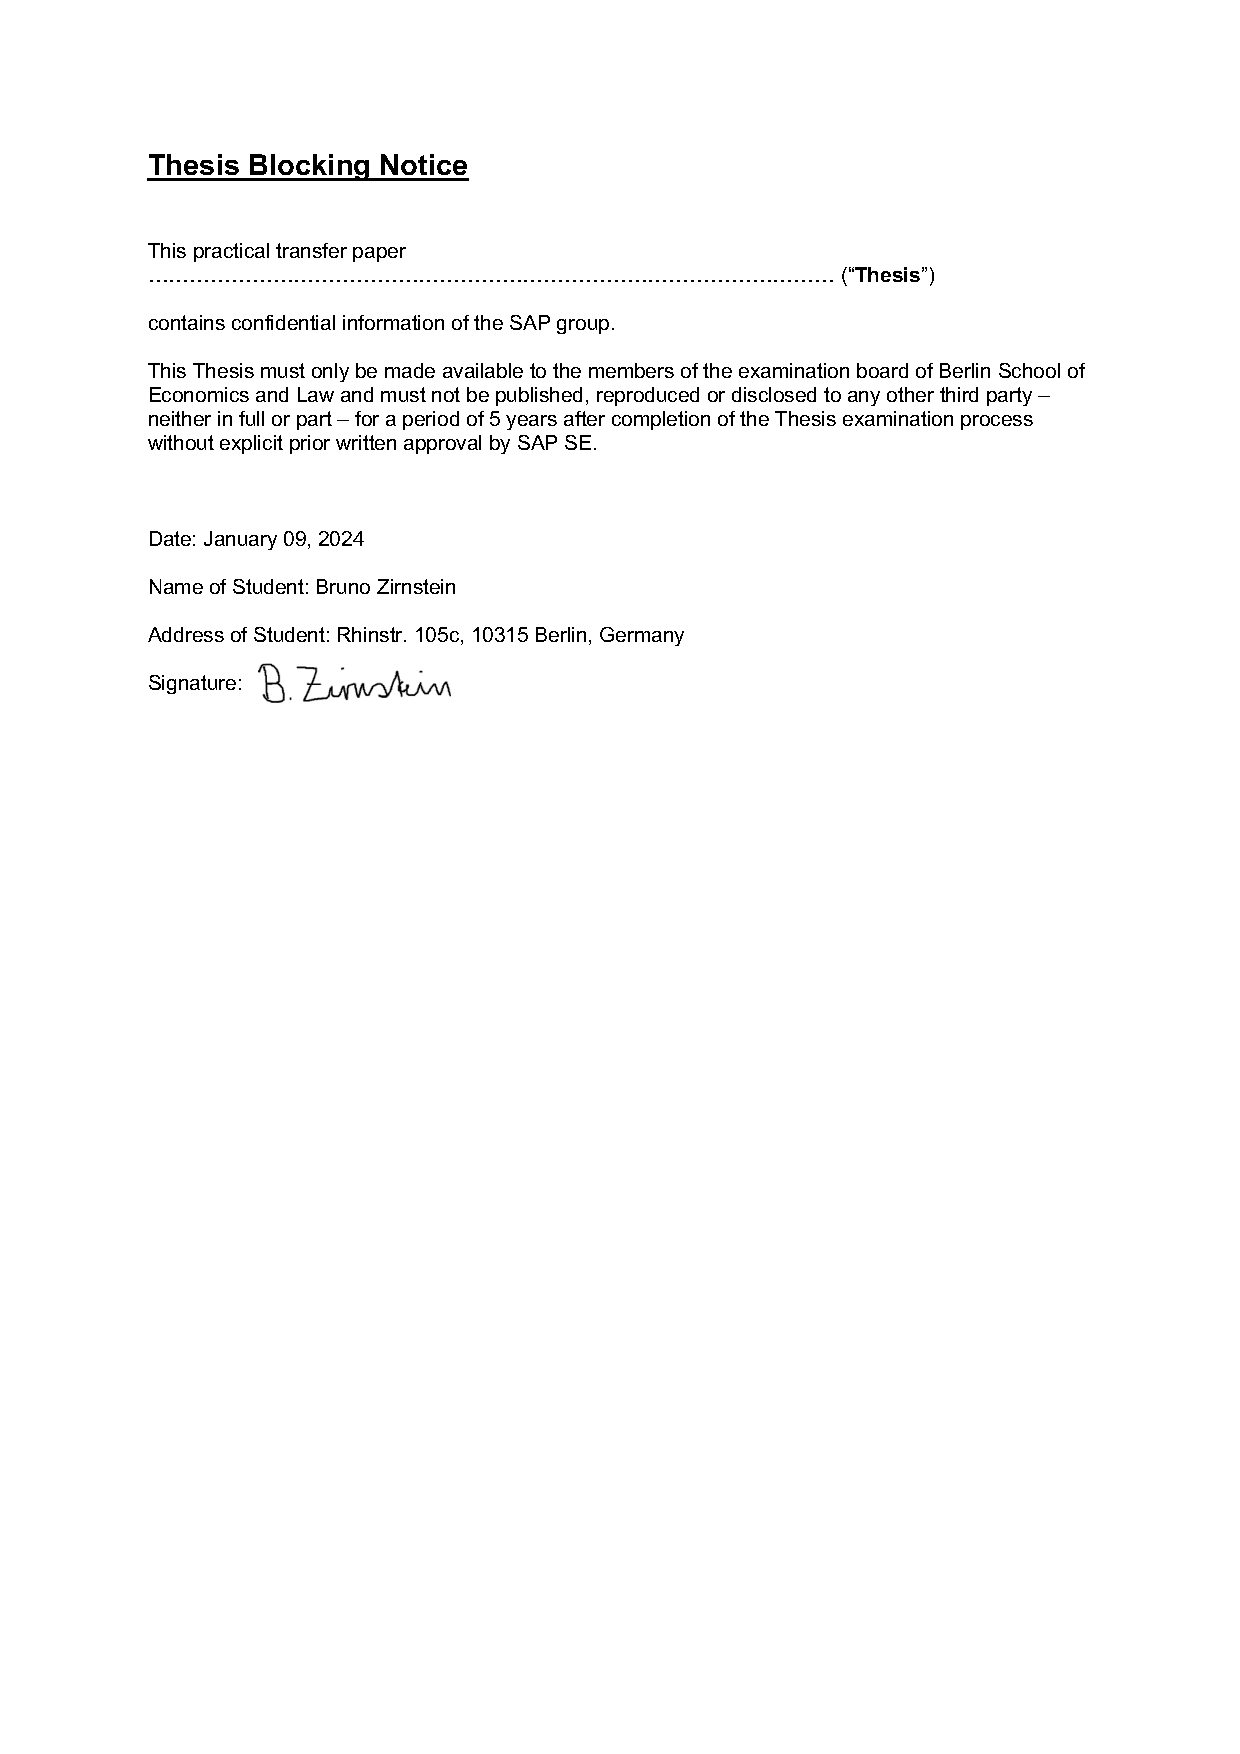
\includepdf[pages=-]{blocking-notice.pdf}
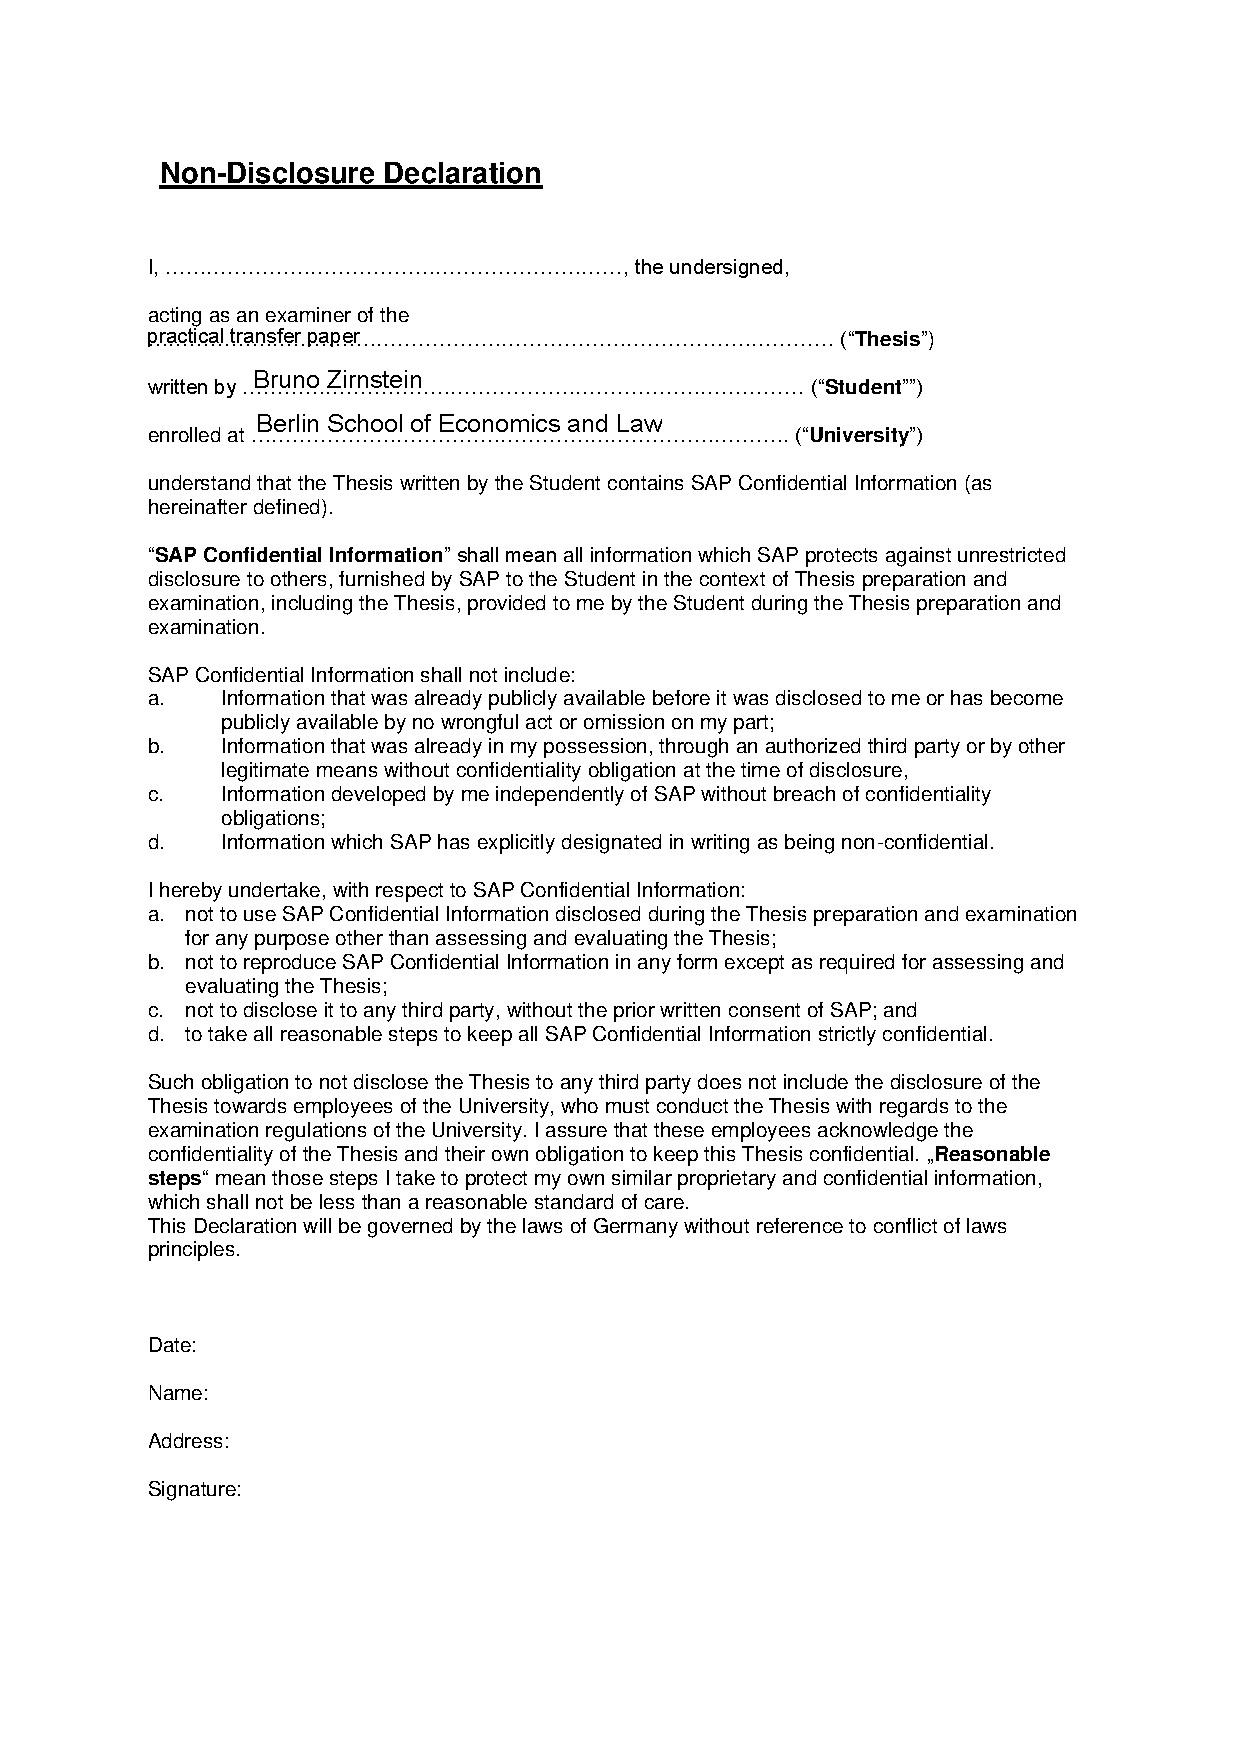
\includepdf[pages=-]{NDA.pdf}

% Titelseite
%%%%%%%%%%%%%%%%%%%%%%%%%%%%%%%%%%%%%%%%%%%%%%%%%%%%%>>>>>>>
%%%%%%%%%%% Titelblatt

%% Anordnung und Aussehen von Titel und Untertitel

\subject{\large\type}

\title{
	\normalfont\endgraf\rule{\textwidth}{.4pt}
	\begingroup
	\centering
	\linespread{1.5}
	\LARGE\topic\\
	% \normalsize\subtopic
	\endgroup
	\endgraf\rule{\textwidth}{.4pt}
}

\date{\normalsize abgegeben am \today\\
	an der \\
	Hochschule für Wirtschaft und Recht Berlin\vspace{5mm}}

\publishers{
	\begin{tabular}{l l}
		\textbf{\normalsize{By: }}                   & \normalsize{\studentName} \tabularnewline
		\textbf{\normalsize{Matriculation number: }} & \normalsize{\matrikelNummer} \tabularnewline
		\textbf{\normalsize{Department:}}            & \normalsize{\fachbereich}  \tabularnewline
		\textbf{\normalsize{Field of study:}}        & \normalsize{\fachrichtung} \tabularnewline
		\textbf{\normalsize{Year of study:}}         & \normalsize{\jahrgang} \tabularnewline
		\textbf{\normalsize{Semester:}}              & \normalsize{\semester} \tabularnewline
		\textbf{\normalsize{Training company:}}      & \normalsize{\company}  \tabularnewline
		\textbf{\normalsize{Evaluating supervisor:}} & \normalsize{\betreuerHS} \tabularnewline
		\textbf{\normalsize{Company supervisor:}}    & \normalsize{\betreuerUnt} \tabularnewline
		\textbf{\normalsize{Word count:}}            & \normalsize{\wordcount} \tabularnewline
		\textbf{\normalsize{Company approval: }}     & \underline{\hspace{4cm}}

		%\textbf{\normalsize{Erstgutachter:}} & \normalsize{\betreuerUnt} \tabularnewline
		%\textbf{\normalsize{Zweitgutachter:}} & \normalsize{\betreuerHS} \tabularnewline
	\end{tabular}
}

\titlehead{
	\begin{center}
		
\includegraphics[scale=0.9]{../assets/images/HWR_Logo_farbig.jpg}
		\hfill
		
\includegraphics[scale=0.9]{../assets/images/SAP_Signavio_Logo.png}
	\end{center}
}

\maketitle

% Seitenabstände für restliches Dokument neu definieren
\newgeometry{verbose,tmargin=4cm,bmargin=2cm,lmargin=21mm,rmargin=3cm}

% Abstract
\newpage
\chapter*{Abstract}
\addcontentsline{toc}{chapter}{Abstract}

This report discusses the extraction of BPMN process models from unstructured textual descriptions by explaining the inherent problems and presenting three distinct approaches to the task. These approaches, leveraging the natural language understanding capabilities of large language models, are evaluated for their ability to create a specific format of BPMN diagram from text-based data. The findings show that the ``Direct Translation'' and ``Intermediate Graph Representation'' approaches present significant challenges and limitations. Contrarily, the ``\nameref*{sec:traces}'' approach proves noteworthy, successfully solving the essential problems of the task while also being easy to implement and offering scope for further development. It therefore is an effective proposition for developing a proof-of-concept.

\onehalfspacing % anderthalbfacher Zeilenabstand
%Inhaltsverzeichnis 
\renewcommand*{\contentsname}{Table of Contents}
\tableofcontents{}
% \addcontentsline{toc}{chapter}{Table of contents}

\clearpage

% \deftranslation[to=German]{Glossary}{Glossar}
% \deftranslation[to=German]{Acronyms}{Akronyme}
\printnoidxglossaries

\clearpage

%%%%Abbildungsverzeichnis(If needed)

\listoffigures
\newpage

%%%%Tabellenverzeichnis(If needed)

% \listoftables
% \newpage

\setcounter{originalpagenumber}{\number\value{page}}
\setcounter{page}{0}
%Arabische Nummrierung 
\pagenumbering{arabic}
% start word counting
%TC:endignore

% Einleitung
\chapter{Motivation}
Large companies usually have structured information about their processes in the format of process models and other artifacts. A large amount of documents containing process-relevant information is however found in an unstructured format such as PDF containing a mixture of diagrams, tables, and free text. A series of qualitative interviews conducted with large enterprises in the DACH region suggests an order of magnitude of 1k to 100k process-relevant documents per company. That's why there is great interest in research and for businesses to develop an approach that can leverage this hidden value by automatically extracting relevant process information into \gls{bpm} software. Such an approach contains multiple components, among others converting textual process descriptions to standardized \acs{bpmn} 2.0 diagrams, which is the topic of this work. The rapid improvements of \acsp{llm} in the past year have given the topic renewed momentum. Moreover, there is generally more interest in the intersection topic of \acsp{llm} and \acs{bpm} \cite{large-process-models}.

%Hauptteil
\chapter{Text-to-Model Problem Statement}
In this chapter, the main challenges of the task are explained, starting with an overview of the overall proposed pipeline, followed by a detailed look at the conversion step.

\section{Extraction Pipeline}\label{sec:pipeline}
In this approach, businesses upload their documents containing process-relevant information. Given these documents, their content is extracted, and all text sections, containing process-relevant information need to be detected and extracted (step 1 in \autoref{fig:pipeline-overview}). It should also be considered to cluster the information per process as there will occur information related to multiple processes in the documents. The process description - respectively a collection of text related to a particular process - can be converted to a \acs{bpmn} 2.0 diagram (step 2 in \autoref{fig:pipeline-overview}), comprehending all relevant information. Then, the generated diagram is rendered in the \acs{ui} for the user to approve it and edit if necessary (step 3 in \autoref{fig:pipeline-overview}). As the last step, the diagram is saved in the user's \gls{signavio-workspace} (step 4 in \autoref{fig:pipeline-overview}).

\begin{figure}[h]
    \centering
    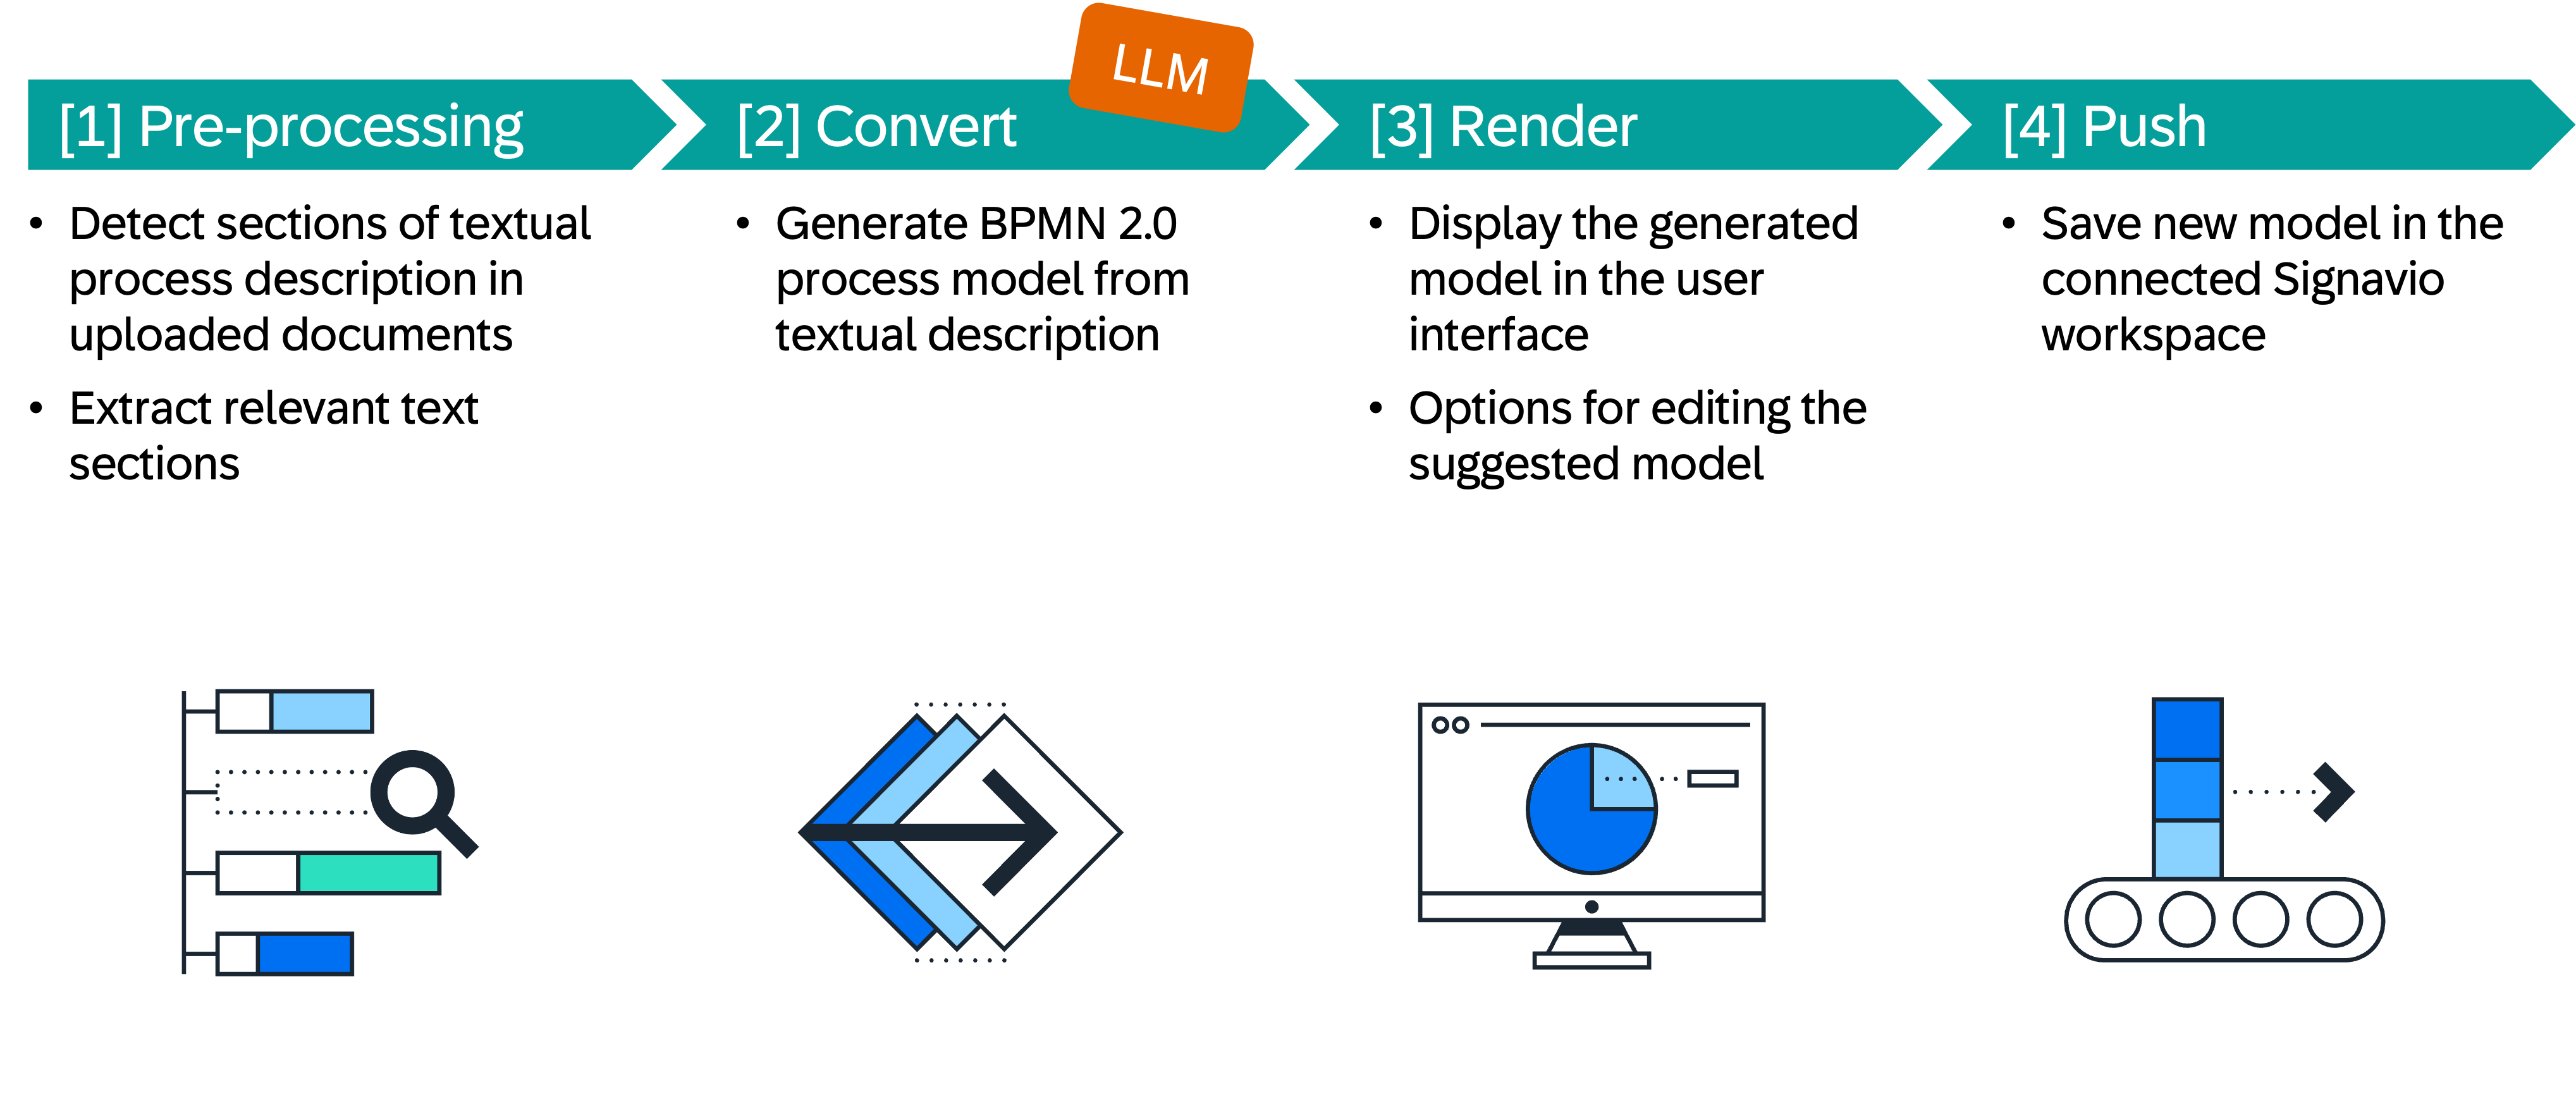
\includegraphics[width=\textwidth,height=\textheight,keepaspectratio]{../assets/images/Text to Model Pipeline.png}
    \caption[Text-to-Model Pipeline Overview]{Text-to-Model Pipeline Overview}
    \label{fig:pipeline-overview}
\end{figure}

\section{Text-to-Model Conversion Step}\label{sec:conversion}
Zooming in on the conversion step of the pipeline - the Text-to-Model transformation - the task can be divided into multiple problems:

\begin{itemize}
    \item Activity extraction
    \item Control flow extraction
    \item Additional information extraction:
          \begin{itemize}
              \item Pools and lanes
              \item Documents
              \item IT-systems
              \item Comments
              \item (Message flow)
          \end{itemize}
    \item \gls{signavio}-compliant output format
    \item Implementation effort (non-functional requirement)
\end{itemize}

\paragraph{Activities \& Control Flow}
First, the essential parts of a \acs{bpmn} 2.0 diagram are activities and the control flow. For the activity extraction, all tasks or subprocesses that are performed in the process need to be identified. Subsequently, an accurate and comprehensive title coherent with the \acs{bpmn} 2.0 guidelines \citep{omg2011bpmn} has to be determined for each activity. For the control flow extraction, the sequence of those activities has to be determined. The control flow can also be split up into multiple branches and joined back together using gateways when different or parallel activity sequences are executed.
% [In that regard, the activity count and control flow complexity should be as minimal as possible to avoid redundant information and duplicate sequence flows.]


\paragraph{Additional Information}\label{par:add-info}
Moreover, the diagram should contain additional information to enhance the information value and detail on certain activities. This feature is not essential for a functioning transformation but would drastically increase the value of the generated diagram. The extraction of the message flow won't be addressed in this work, because it is not of high importance for \gls{signavio} users.

\paragraph{Output Format}
Lastly, to save the process model in the connected \gls{signavio-workspace}, the output must be code for a \acs{bpmn} 2.0 diagram, complying with a certain \gls{signavio}-specific format (see \autoref{fig:code-example} for an example). Therefore, the result of the conversion step cannot be any other format, which might be easier to achieve.

\paragraph{Implementation Effort}
As an additional (non-functional) requirement the implementation effort has to be considered. As the context of this work is an innovation project, the resources for testing and implementing approaches are very limited. The primary objective of the project is the development of a \glsentrylong{poc} and the demonstration of feasibility. Therefore, it is crucial to keep the effort to a minimum.

% \chapter{Related work \& Collaboration}\label{chapter:related-work}
\chapter{Related work}\label{chapter:related-work}
Scientific interest and work on the task of transforming natural language into a formal process representation has existed for over 10 years \citep{process-extraction-from-text}. Various approaches from the \acs{nlp} area were investigated to solve this problem \citep{investigation-text-to-bpmn}. However, with the advancements of \gls{llm} capabilities, the \acs{nlp} area was reformed and new approaches have emerged. Still, not many papers investigating these new approaches were published.

\citeauthor{conversational-process-modelling} explore the topic of chatbot-assisted conversational process modeling \citep{conversational-process-modelling}. Among other aspects, their work includes the extraction of tasks and the control flow from a process description using \glspl{llm} and a proposed set of \acsp{kpi} for comparing generated with ground-truth models in an evaluation step. Other work investigates the extraction of business process elements from text \cite{text-to-bp-elem} and the transformation of textual process information to intermediate formats \cite{text-to-inter-rep}.

% Among discussing my work with other \gls{signavio} researcher, I collaborate with Dr. Timotheus Kampik, Adjunct Associate Professor at the Umeå University in Sweden and Principal Scientist in Residence at \gls{signavio}.


\chapter{Approaches to Text-to-Model}
In this chapter, three approaches using the unique natural language understanding capabilities of \acsp{llm} are presented and assessed.

\section{Direct Translation}\label{sec:direct-translation}
\paragraph{Concept}
The most straightforward approach is to directly transform the given process description into \gls{signavio}-compliant \acs{bpmn} 2.0 \acs{json} code\footnote{This \acs{json} code is how \acs{bpmn} 2.0 diagrams can be represented at \gls{signavio} and used in its software. It therefore is the desired output format.} with a single request to an \gls{llm}. This approach is efficient in terms of implementation effort and runtime.

\paragraph{Results}
To test this approach, \acs{gpt}-4 was one-shot prompted to generate such \gls{signavio}-compliant \acs{json} code given a process description. However, the results were not satisfying as the generated code was not in the specified format. The desired format is very complex as it contains a lot of details about the diagram like specific \acsp{id} and explicit coordinates for each graphical element of the diagram (see \autoref{fig:code-example}). Therefore, the \gls{llm} seems to have trouble with generating compliant code. The approach is not further investigated as it fails to meet a key requirement.

% [There are alternative approaches to the direct translation. For example, specifying a simpler \acs{bpmn} 2.0 \acs{json} output format for the \gls{llm} and transforming the simpler one into the \gls{signavio}-compliant format in a second step. Testing that alternative with the same setup as above and a simliar prompt, \acs{gpt}-4 was able to output the specified simpler format correctly. That second step however would require a lot of effort and therefore was not investigated further as there are limited resources to the project.]

\section{Intermediate Graph Representation}\label{sec:mermaid-approach}
\paragraph{Concept}
Another approach is to transform the process description into another (simpler) intermediate format, such as a graph representation, which is transformed into \gls{signavio}-compliant code in an extra step. This might work better than the first approach because the \gls{llm} only needs to understand the simpler intermediate representation, for example, the format of ``Mermaid.js''\cite{mermaid-js} code (example in Figures \ref{lst:mermaid-example-code} and \ref{fig:mermaid-example-graph}).

\paragraph{Results}
Testing the first step of this approach (see the prompt in \autoref{lst:mermaid-prompt}), \acs{gpt}-4 was able to generate valid code for a Mermaid.js graph, with elements similar to \acs{bpmn} 2.0 (see \autoref{lst:mermaid-test-input} and \autoref{fig:mermaid-test-output} for an example input and output of the first step). As \autoref{fig:mermaid-test-output} demonstrates, there are some flaws in the generated diagram. For example, there are two duplicate sequence flows that could be joined back together using a gateway and there are also missing end nodes. To summarize, the first step requires further optimization, and the second conversion step from the intermediate format to the \gls{signavio}-compliant code is required. It might be a viable approach, but it requires too much effort and therefore won't be further investigated for now.

\section{Generating Traces \& Process Mining}\label{sec:traces}
\paragraph{Concept}
Looking at the generated Mermaid.js graph in \autoref{fig:mermaid-test-output}, the generated diagram isn't a comprehensive process representation but rather displays all possible activity sequences. With this in mind, the idea of the third approach is to generate a unique set of \glspl{trace} from the process description and use a \gls{process discovery algorithm} to extract a process model from that.

In the first step, \acs{gpt}-4 is prompted to extract and output a unique set of \glspl{trace} given the process description. The output is a list of \glspl{trace} (see \autoref{lst:traces-example} for an example), which are then used as an (artificial) \gls{event log} and fed into the ``Split Miner'' \citep{split-miner} algorithm that extracts the process model and returns it as compliant code. The Split Miner algorithm is a state-of-the-art \gls{process discovery algorithm} from 2019 that is implemented in an existing \gls{signavio} service. Therefore, the approach is little effort and always returns \gls{signavio}-compliant \acs{json} code for a \acs{bpmn} 2.0 diagram.

\paragraph{Results}Testing this approach (see the prompt for \gls{trace} extraction in \autoref{lst:traces-prompt}), \acs{gpt}-4 reliably extracts a coherent and unique set of \glspl{trace}; the Split Miner service outputs a \gls{signavio}-compliant diagram (see an exemplary result in \autoref{fig:traces-test-output}).

\begin{figure}[h]
    \centering
    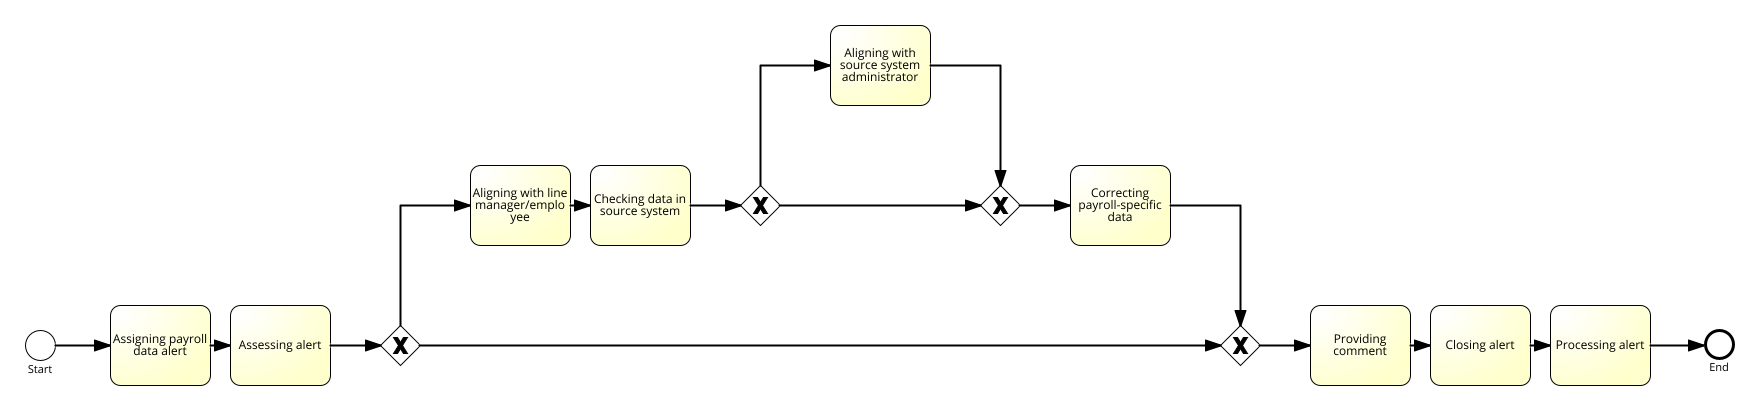
\includegraphics[width=\textwidth,height=\textheight,keepaspectratio]{../assets/images/Traces Test Output.png}
    \caption{Generated \gls{signavio} \acs{bpmn} 2.0 diagram using the \nameref{sec:traces} approach}
    \label{fig:traces-test-output}

    \medskip
    \small
    See the process description used as input in \autoref{lst:traces-test-input} and the generated \glspl{trace} (artificial \gls{event log}) in \autoref{lst:traces-test-traces}.
\end{figure}

For various process descriptions, with similar structure, syntax, and complexity to the one shown in \autoref{lst:traces-test-input}, the output diagram always contains all referenced activities and the correct control flow, represented by activities, exclusive gateways, a start, and an end node.

For process descriptions that are more ambiguous, implicit, and complex (see example in \autoref{lst:hard-description}), the current implementation of the approach struggles to extract complex control flows perfectly. Partially, the assumption of implicit knowledge is missing. However, that doesn't mean it can't deal with more difficult process descriptions, but the approach has to be fine-tuned, e.g. by optimizing prompts and covering certain edge cases.


\chapter{Evaluation}
To systematically assess the performance of any conversion approach, its generated diagram has to be evaluated for various process descriptions of different complexities. The evaluation can be done by an expert in process modeling, who manually compares the generated diagram with the original process description in terms of extracted activities, control flow, and additional information.

If there was a dataset of process descriptions with matching \acs{bpmn} 2.0 diagrams given, another possibility is to compare the diagram generated from the process description with the matching diagram from the dataset. This \textit{round-trip} evaluation can also be performed automatically. Therefore, a set of formal metrics to measure the conformance of the two diagrams need to be defined \cite{bpmn2-comformance, bpmn-event-log-conformance-checking, bpmn-conformance}. This automatic round-trip evaluation could be more accurate by reducing manual errors and biases and would allow different approaches to be formally evaluated as well as each part of an approach to be optimized against an objective score. However, it also requires additional preliminary effort and an appropriate dataset, which is not trivial. For example, many different diagrams are valid ground-truth diagrams for one process description. This especially applies to complex and ambiguous descriptions assuming much implicit knowledge \cite{process-model-ambiguity}.

As the purpose of this work is to investigate approaches that can solve the crucial problems of the described task in the first place, that's how approaches are evaluated. Any further evaluation techniques are not the topic of this work.

\chapter{Prototype Implementation}
The Mermaid.js and \nameref{sec:traces} approaches were implemented as prototypes, showcasing the functionality and the current progress to other internal stakeholders. Both prototypes were built as a web application with Python 3.11 \cite{python3} and the open-source library Streamlit \cite{streamlit}. For using \acs{gpt}-4, both prototypes use \gls{sap}'s \acs{btp} \acs{llm} Proxy Service, \gls{sap}'s service for \acs{llm} usage that uses Microsoft's Azure OpenAI Service \cite{azure-openai} in the background. The Mermaid.js approach prototype can be run locally (see screenshot of the prototype in \autoref{fig:mermaid-prototype}). As the \nameref{sec:traces} approach is more promising, this prototype was made available internally. It is deployed on \gls{sap}'s \gls{btp}, hosted by Cloud Foundry (see screenshot of the prototype in \autoref{fig:trace-prototype}).


\begin{figure}[h]
    \centering
    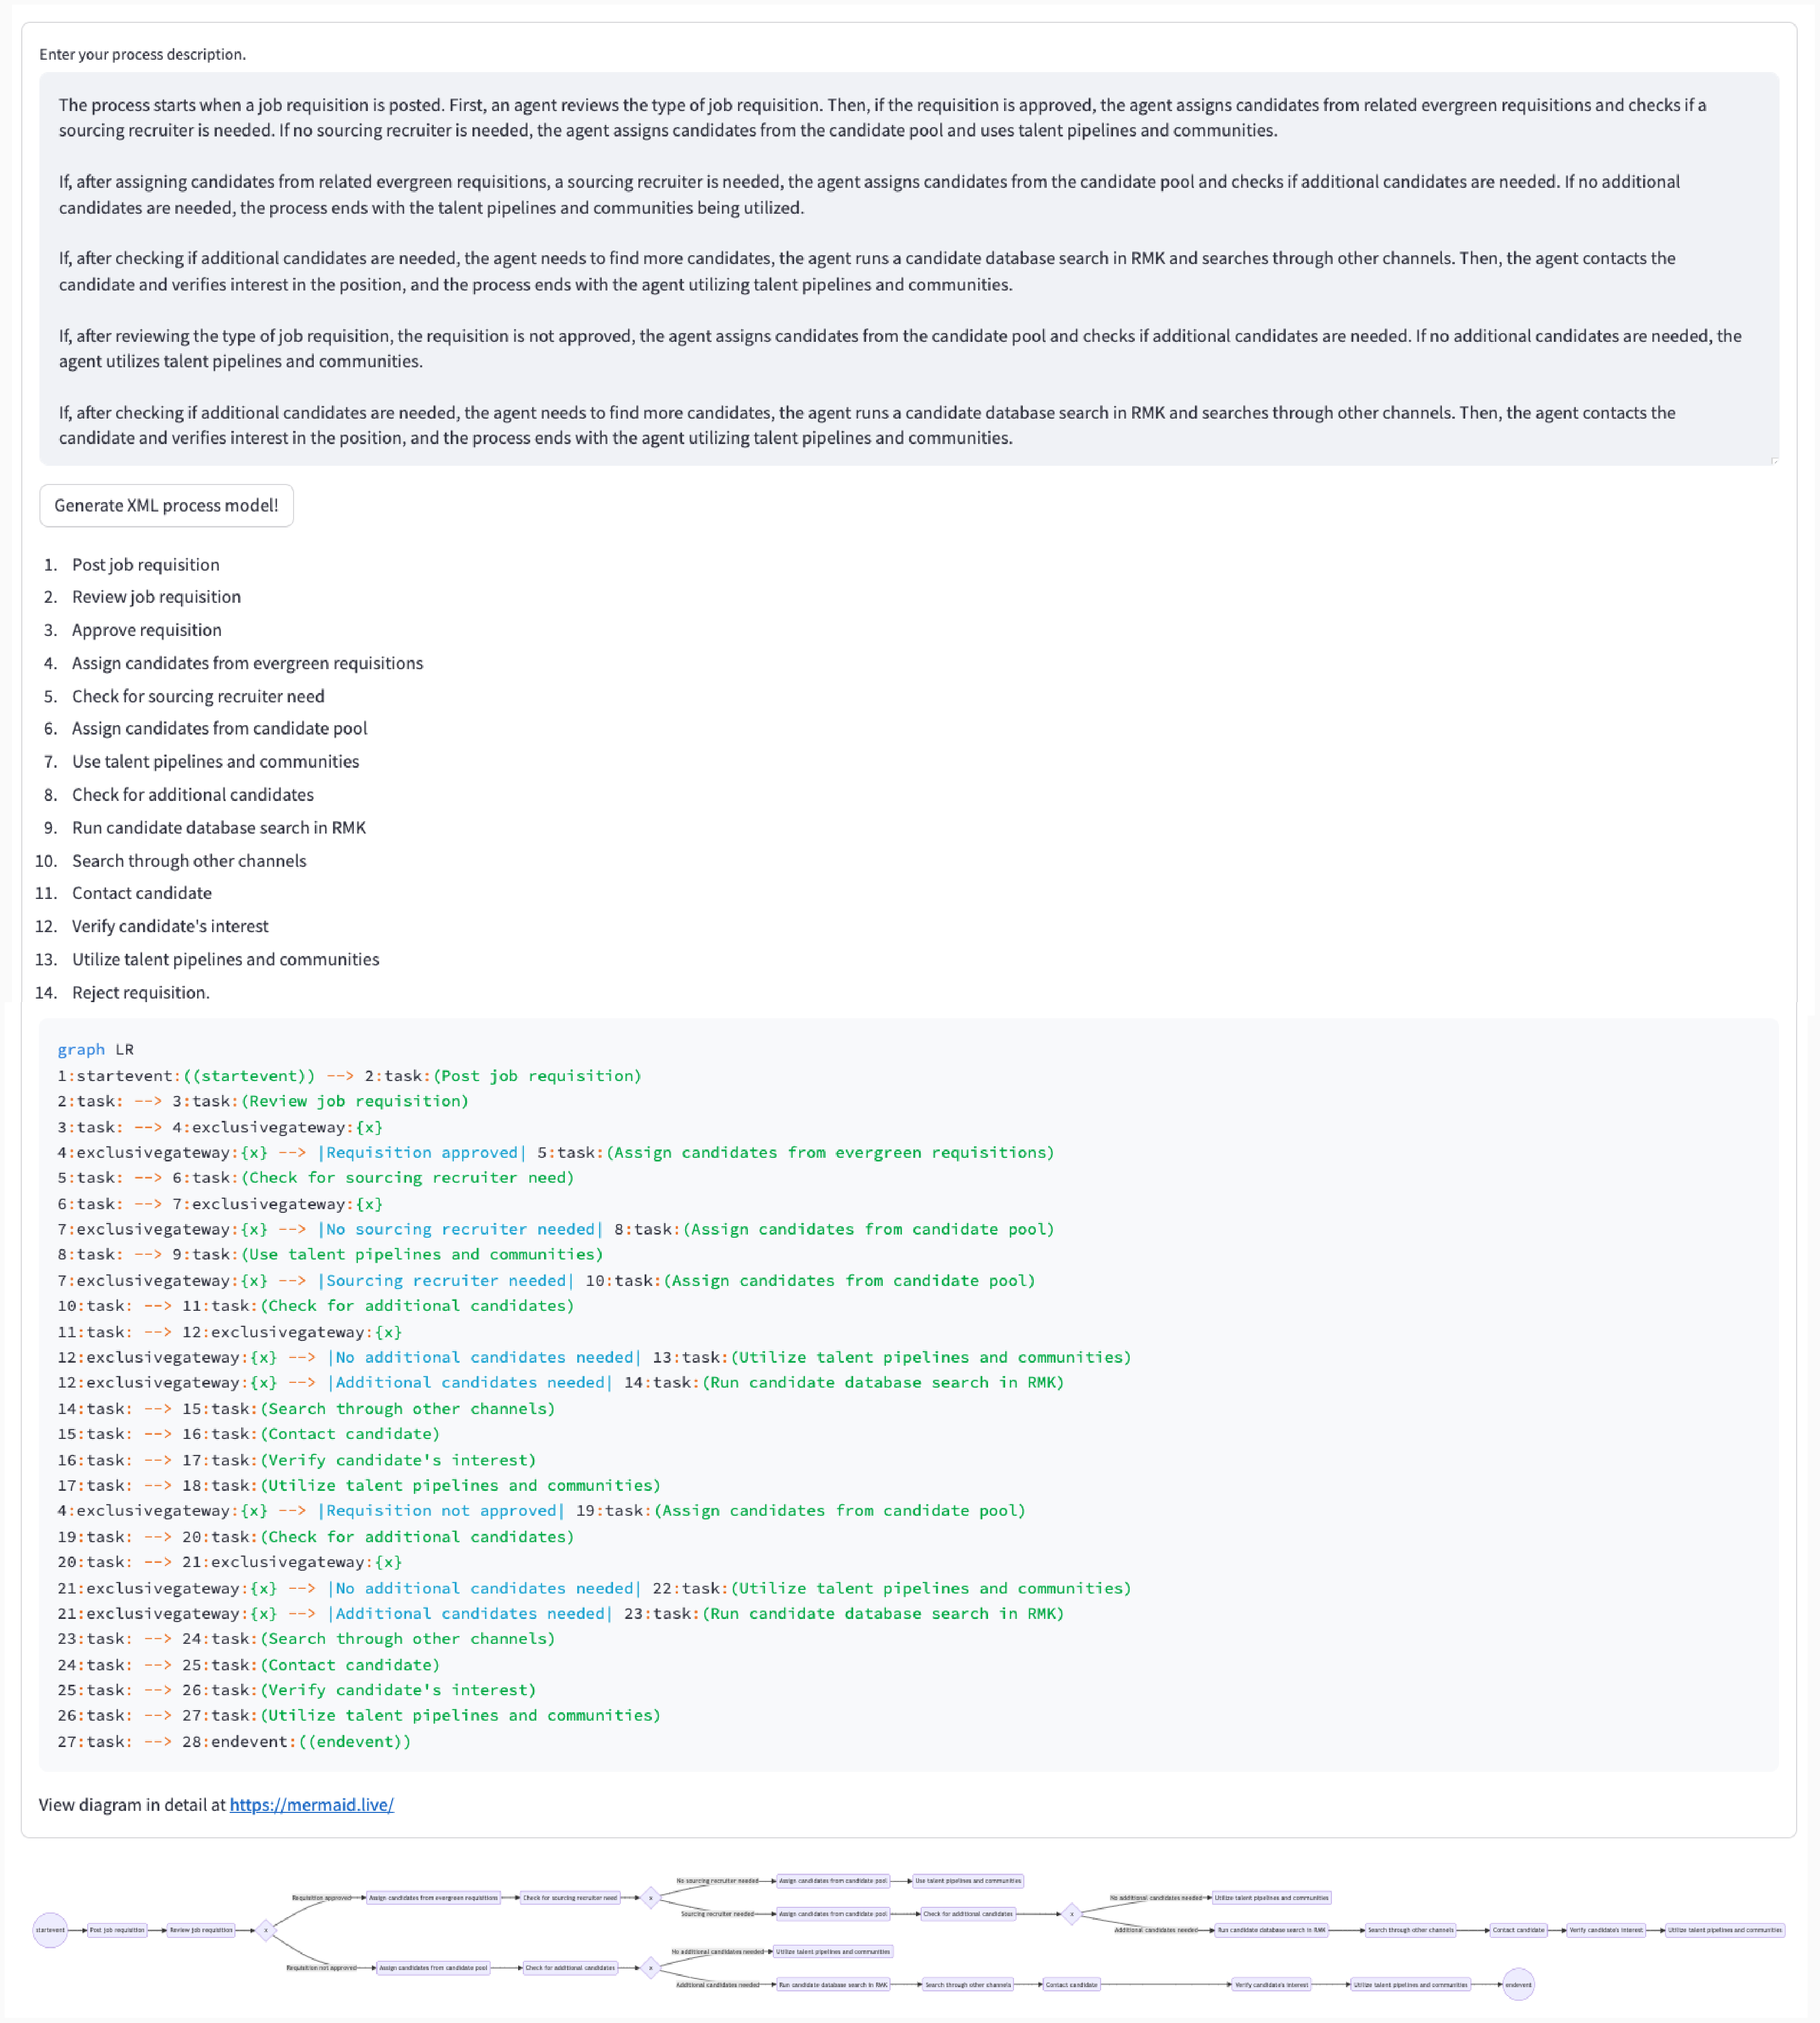
\includegraphics[width=\textwidth,height=\textheight,keepaspectratio]{../assets/images/Mermaid prototype.png}
    \caption{Screenshot of the Mermaid.js approach prototype}
    \label{fig:mermaid-prototype}

    \medskip
    \small
    See the outputted graph also  in \autoref{fig:mermaid-test-output}.
\end{figure}

\begin{figure}[h]
    \centering
    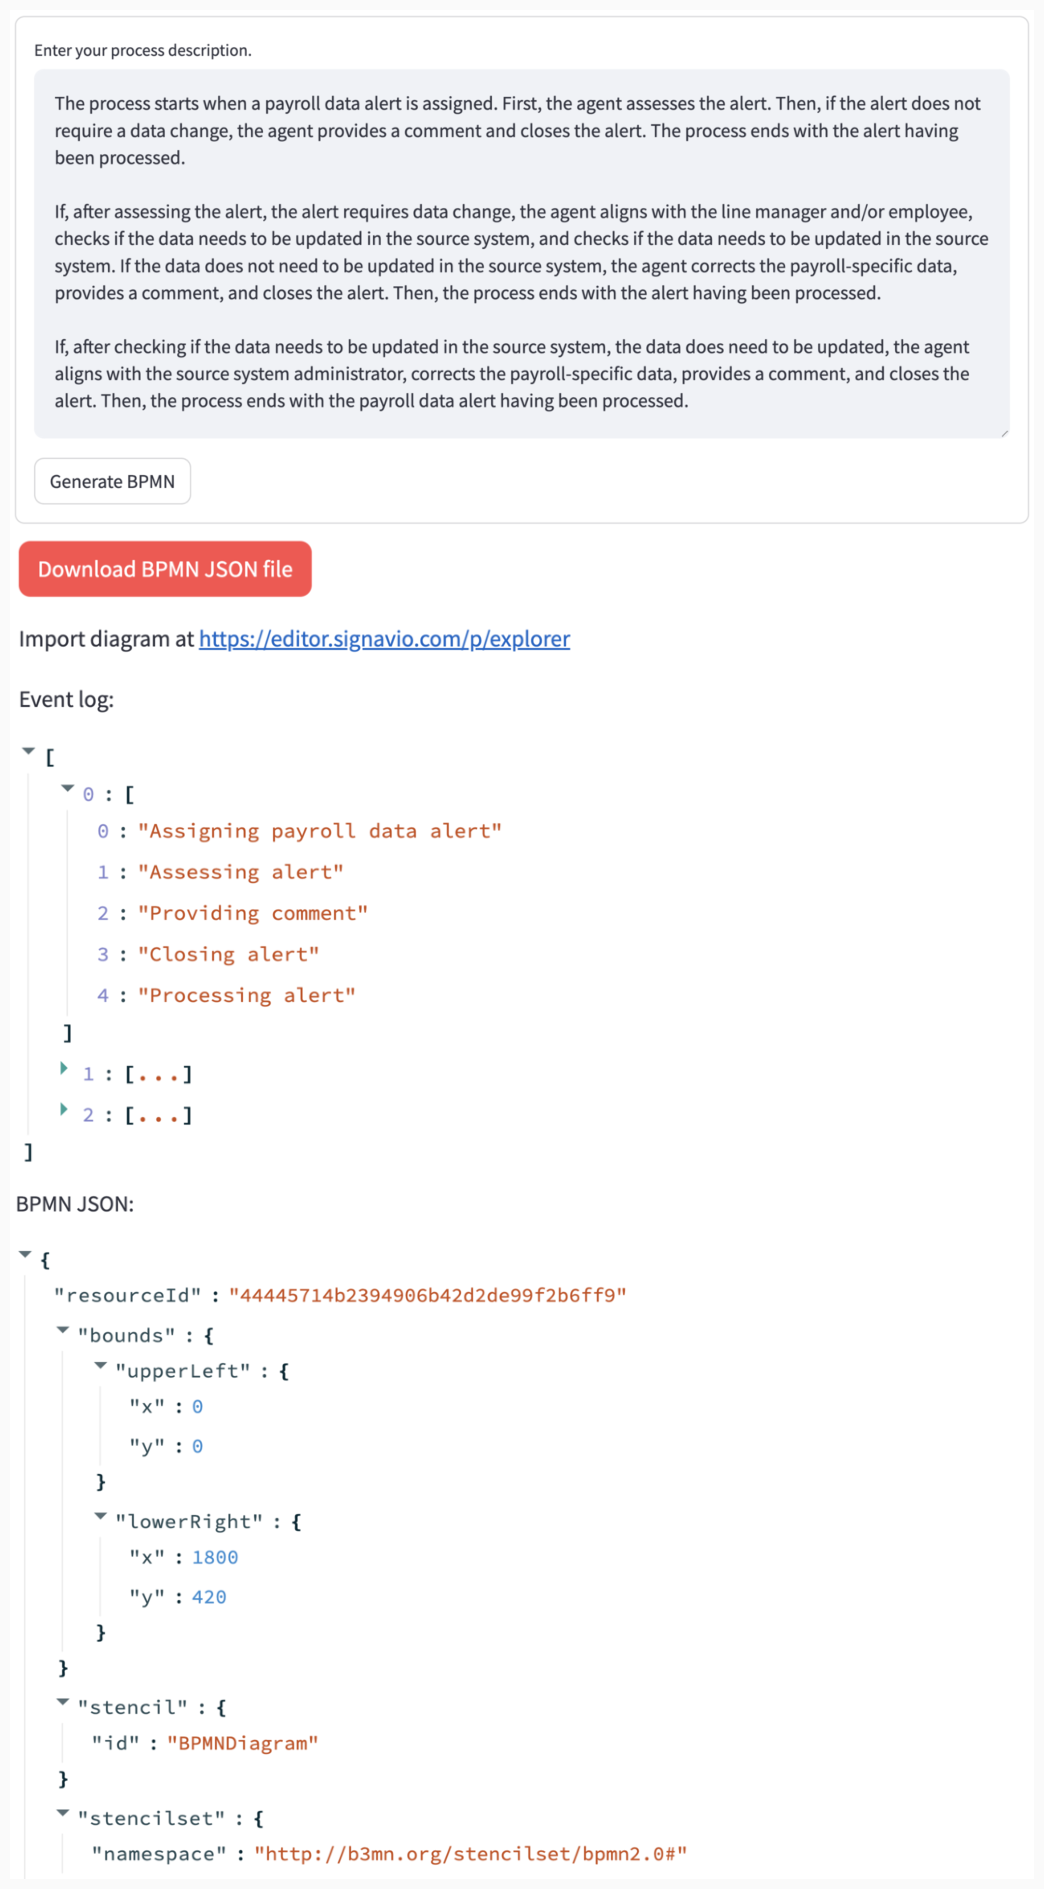
\includegraphics[height=0.95\textheight,keepaspectratio]{../assets/images/Trace prototype.png}
    \caption{Screenshot of the \nameref{sec:traces} approach prototype}
    \label{fig:trace-prototype}

    \medskip
    \small
    See the outputted diagram in \autoref{fig:traces-test-output}.
\end{figure}

\chapter{Discussion}
\paragraph{Summary}
Aggregating all results, the approaches \nameref{sec:direct-translation} and \nameref{sec:mermaid-approach} are not suitable for the current \acs{poc} project. However, the \nameref{sec:traces} approach solves all the crucial problems of the task. It extracts the activities and the control flow and always outputs \gls{signavio}-compliant \acs{bpmn} 2.0 \acs{json} code. The approach is also very efficient in terms of implementation effort as all its functionality is handled by two existing services (\acs{gpt}-4 and the \gls{signavio} Split Miner service). Meanwhile, it does not extract additional information as described in the \hyperref[par:add-info]{problem statement} and still struggles with more difficult process descriptions. But, the approach also leaves room for further development and improvement (see \nameref{par:next-steps}). It therefore is a viable solution for the development of a \acs{poc}.


\paragraph{Future Work}\label{par:next-steps}
Some next steps regarding the \nameref{sec:traces} approach that can be the subject of future work are:

\begin{itemize}
    \item Add a post-processing step to enhance the diagram with additional information using another \gls{llm} request, given the process description and generated diagram code
    \item Gather more (diverse) process descriptions to systematically examine edge cases and malfunctions
    \item Implement an automated round-trip evaluation after defining a set of formal metrics
    \item Optimize the used prompts and assess the application of prompt chaining
    \item Experiment with human-in-the-loop approaches:
          \begin{itemize}
              \item Suggest multiple possible process variants and allow the user to select
              \item Allow the user to edit extracted \glspl{trace}, following conversational modeling \cite{conversational-process-modelling}
          \end{itemize}
\end{itemize}

The work, presented in this report will be continued and advanced.

% add: survey about most used BPMN components / elements, add to section above that explains that message flow is not that important

%Schluss
\chapter{Conclusion}
In conclusion, the task of extracting BPMN process models from unstructured textual descriptions was investigated, motivated by the need of large companies to leverage their hidden process knowledge stored in internal documents. Three different approaches using \glspl{llm} were presented and assessed, namely Direct Translation, Intermediate Graph Representation, and \nameref*{sec:traces}.

The first two approaches were not feasible for the current \glsentrylong{poc} project, as they required too much effort and failed to produce a compliant output format. The  \nameref*{sec:traces} approach, on the other hand, was able to solve the crucial problems of the task, such as extracting the activities and the control flow, always outputting Signavio-compliant \acs{json} code and being very efficient in terms of implementation effort. However, the approach does not extract additional information and still struggles with more difficult process descriptions, but it also leaves room for further development and improvement.

\newpage

\pagenumbering{Roman}
\setcounter{page}{\number\value{originalpagenumber}}

%TC:ignore

%Literaturverzeichnis
% \addtocontents{toc}{\protect\vspace*{\baselineskip}}
\nocite{*}
\bibliographystyle{abbrvnat}
\bibliography{../assets/literature/sources}

\newpage

%Anhang
\appendix
\chapter*{Appendix}
\addcontentsline{toc}{chapter}{Appendix}

\begin{figure}[h]
    \lstinputlisting{../assets/mermaid-example.txt}
    \caption{Example Mermaid.js code for the graph in \autoref{fig:mermaid-example-graph}}
    \label{lst:mermaid-example-code}
\end{figure}

\hspace{3cm}

\begin{figure}[h]
    \centering
    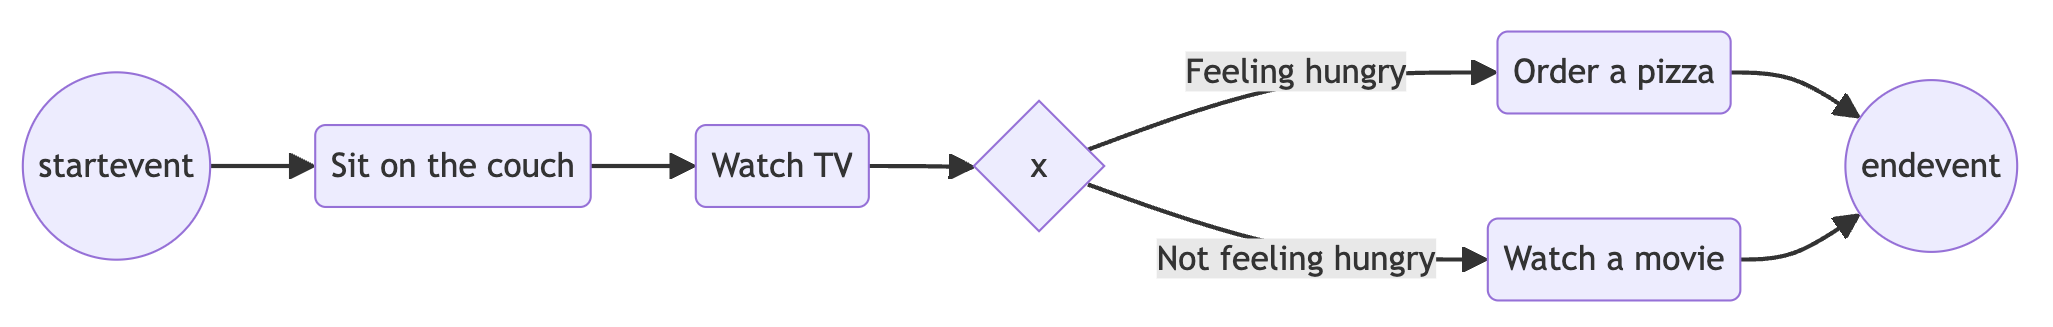
\includegraphics[width=\textwidth,keepaspectratio]{../assets/images/Mermaid Graph Example.png}
    \caption{Example Mermaid.js graph for code in \autoref{lst:mermaid-example-code}}
    \label{fig:mermaid-example-graph}
\end{figure}

\begin{figure}[h]
    \centering
    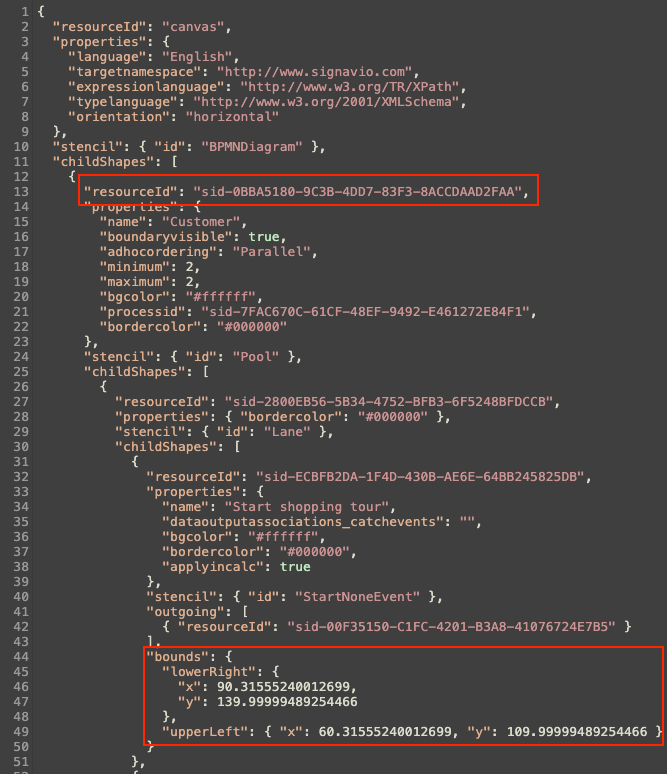
\includegraphics[width=\textwidth,height=\textheight,keepaspectratio]{../assets/images/Supermarket Shopping Signavio BPMN JSON Code Example.png}
    \caption{Extract of \gls{signavio}-compliant \acs{bpmn} 2.0 \acs{json} Code}
    \label{fig:code-example}

    \medskip
    \small
    The first 50 lines of the \acs{json} code are shown. A contained \acs{id} and the included coordinates of an element are highlighted. In the following code (not shown), more \acs{bpmn} 2.0 elements follow as part of the ``childShapes'' array in line 25 as well as an array of associations.
\end{figure}


\begin{figure}[h]
    \lstinputlisting[basicstyle=\scriptsize]{../assets/mermaid-code-prompt.txt}
    \caption{Prompt for generating a Mermaid.js graph}
    \label{lst:mermaid-prompt}
\end{figure}

\begin{figure}[h]
    \lstinputlisting[basicstyle=\scriptsize]{../assets/process-description-transcriber-1.txt}
    \caption{Example process description}
    \label{lst:mermaid-test-input}

    \medskip
    \small
    Used as input to evaluate the Mermaid.js approach (see \autoref{sec:mermaid-approach}). See the generated output in \autoref{fig:mermaid-test-output}.
\end{figure}


\begin{landscape}
    \begin{figure}[h]
        \centering
        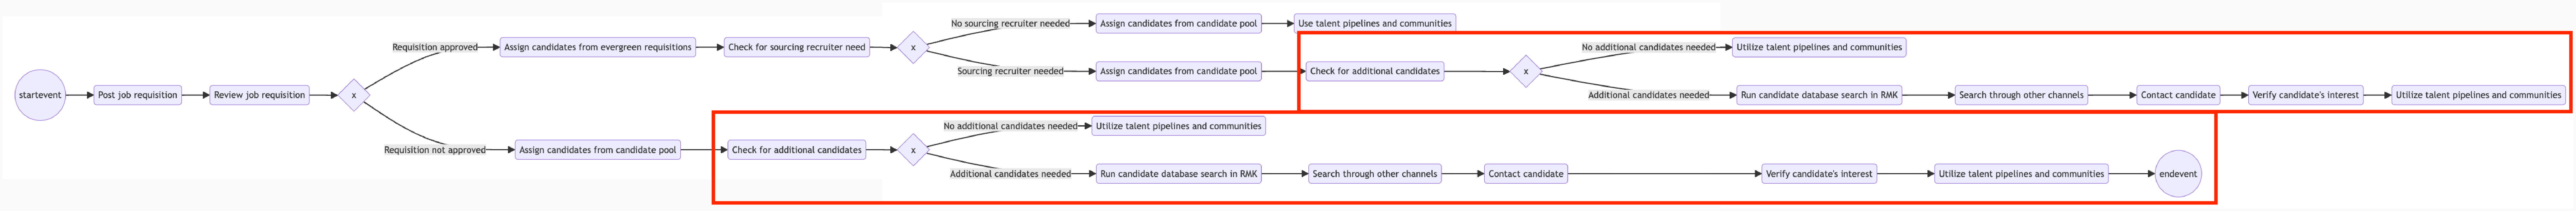
\includegraphics[width=\textheight,keepaspectratio]{../assets/images/Mermaid Test Output.png}
        \caption{Generated Mermaid.js graph}
        \label{fig:mermaid-test-output}

        \medskip
        \small
        Output of the Mermaid.js approach (see \autoref{sec:mermaid-approach}) for the process description in \autoref{lst:mermaid-test-input}. Two duplicate sequence flows are highlighted.
    \end{figure}
\end{landscape}

\begin{figure}[h]
    \lstinputlisting[basicstyle=\scriptsize]{../assets/traces-prompt.txt}
    \caption{Prompt for extracting a unique set of \glspl{trace} from a process description}
    \label{lst:traces-prompt}
\end{figure}

\begin{figure}[h]
    \lstinputlisting[basicstyle=\scriptsize]{../assets/traces-example.txt}
    \caption{Example of a unique set of \glspl{trace}.}
    \label{lst:traces-example}
\end{figure}

\begin{figure}[h]
    \lstinputlisting[basicstyle=\scriptsize]{../assets/traces-test-input.txt}
    \caption{Tested input process description for diagram in \autoref{fig:traces-test-output}.}
    \label{lst:traces-test-input}
\end{figure}

\begin{figure}[h]
    \lstinputlisting[basicstyle=\scriptsize]{../assets/traces-test-traces.txt}
    \caption{Generated set of traces (artificial \gls{event log}) for the input process description in \autoref{lst:traces-test-input}.}
    \label{lst:traces-test-traces}
\end{figure}

\begin{figure}[h]
    \lstinputlisting[basicstyle=\scriptsize]{../assets/hard-process-description.txt}
    \caption{Example of a more complex process description}
    \label{lst:hard-description}
\end{figure}

%Ehrenwörtlich erklährung 
\chapter*{Declaration of Authorship}
\addcontentsline{toc}{chapter}{Declaration of Authorship}

% Hier der offizielle Text der eidesstattlichen Erklärung
I hereby declare that the thesis submitted is my own unaided work. All direct or indirect sources used are acknowledged as references. I am aware that the thesis in digital form can be examined for the use of unauthorized aid and in order to determine whether the thesis as a whole or parts incorporated in it may be deemed as plagiarism. For the comparison of my work with existing sources, I agree that it shall be entered in a database where it shall also remain after examination, to enable comparison with future theses submitted. Further rights of reproduction and usage, however, are not granted here.

This paper was not previously presented to another examination board and has not been published.
% Etwas Abstand für die Unterschrift
\vspace{2cm}

% Hier kommt die Unterschrift drüber
\begin{tabular}{lp{4em}l}
    \hspace{5cm} &  & \hspace{3.5cm}        \\\cline{1-1}\cline{3-3}
    City, date   &  & \studentName \newline
\end{tabular}

%TC:endignore
\end{document}
